\documentclass[a4paper,10pt,twocolumn]{article}
\usepackage[margin=1.75cm,columnsep=0.65cm]{geometry}
\usepackage[T1]{fontenc}
\usepackage{lmodern,microtype,amsmath,booktabs,array,graphicx}
\usepackage[hidelinks]{hyperref}
\usepackage{url}
\usepackage{flushend}
\usepackage{tikz}
\usetikzlibrary{arrows.meta,positioning,fit,calc,backgrounds}
\setlength{\parskip}{2pt}
\setlength{\parindent}{1em}
\setlength{\textfloatsep}{9pt}
\raggedbottom
\title{A Reference Architecture for Building Domain-Specific Retrieval-Augmented Conversational Assistants}
\author{Stefan Milev\\\small Faculty of Computer Science and Engineering\\\small Ss. Cyril and Methodius University in Skopje\\\small Supervisor: Prof. Dr. Riste Stojanov}
\date{}
\begin{document}
\maketitle
\begin{abstract}
We evaluate how effectively a student-support chatbot answers questions and provides useful guidance, and use its design to propose a reference architecture. After a 20-case pilot, we test 96 historical email questions and 96 selectively logged chatbot questions. The test reuses deployed retrieval and prompt code with controlled Luna generation; it excludes live agents, tools and conversation history. With a shared retrieval threshold and no fallback, the AI judge labels 31/96 email responses and 53/96 chatbot responses as supported answers or useful routing. Twenty of the 25 chatbot supported-answer labels use references with no retained facts, so they do not establish factual accuracy. Separate FAQ/document thresholds change assistance totals to 30/96 and 52/96. A second, 40-question email comparison uses an expanded document collection, reference answers and a prompt that checks source applicability and procedural steps. Initial strict-completion labels show a five-point gain, which becomes a 2.5-point decline when the assessment receives the full generation evidence; the latter 95\% paired interval is $[-12.5,7.5]$. Neither comparison establishes better assistance. The findings identify missing evidence and assessment errors, rather than a verified success rate for the deployed system.
\end{abstract}
\par\noindent\textbf{Keywords:} retrieval-augmented generation; reference architecture; university support; Macedonian; automated assessment.

\section{Introduction}
University support involves FAQs, regulations, changing timetables, and individual requests that require private records or institutional decisions. A chatbot needs suitable evidence to answer these questions. It must also make clear when it is explaining a procedure and when the user still needs to contact staff or complete an official process.

The finki-hub chatbot serves students at the Faculty of Computer Science and Engineering (FCSE), Ss. Cyril and Methodius University in Skopje. The questions include Macedonian written in Cyrillic or Latin transliteration, as well as English. The system combines FAQ and document retrieval with tools for structured information. Separating source preparation, retrieval, answer generation, delivery and monitoring makes it possible to trace errors and test changes to individual components.

The central question is whether the assistant gives students a supported and sufficiently complete answer, or useful guidance when a direct answer is inappropriate. We examine these outcomes on questions drawn from university correspondence and chatbot logs. Architecture explains how sources reach the answer; a controlled retrieval comparison tests whether changing that evidence improves assistance. A shared minimum reranker score treats FAQs and document passages alike, although they differ in length and format. We test a lower document threshold and a fallback that keeps the best candidate when none reaches the threshold, separately and together.

We contribute an evaluation on real university questions and a reference architecture based on the implemented system. The architecture separates three tasks: loading content while recording its source, selecting evidence for an answer, and delivering responses through web and Discord interfaces. We propose reusing these interfaces elsewhere, but do not test that reuse. The evaluation asks three questions:
\begin{description}
\item[RQ1:] How often does the judge label responses as supported answers or useful routing, and what problems remain?
\item[RQ2:] How do separate score thresholds and fallback affect these outcomes when generation settings stay fixed?
\item[RQ3:] How do the question sample and AI judge limit conclusions about effectiveness?
\end{description}
The architecture explains the tested path. We do not compare competing system designs.

\section{Background and related work}
Retrieval-augmented generation (RAG) uses external evidence to generate an answer~\cite{lewis2020rag}. Dense passage retrieval compares vectors (embeddings) of questions and passages, learned so that similar texts get similar embeddings, to find candidates~\cite{karpukhin2020dpr}, and a cross-encoder (our reranker) can then score each question and passage together~\cite{nogueira2019bertrerank}. M3-Embedding (the BGE-M3 model) supports multiple languages, retrieval methods and text lengths~\cite{chen2024m3}. It is built on XLM-RoBERTa, whose training data include Macedonian~\cite{conneau2020xlmr}, and our recall analysis is the only Macedonian test of it we know of (Section~\ref{sec:live}). We use these methods, but their published benchmark results do not measure performance on FCSE student questions. Multilingual benchmarks such as MIRACL (a retrieval test set in 18 languages)~\cite{zhang2023miracl} and NoMIRACL~\cite{thakur2024nomiracl} and work on Macedonian models and corpora~\cite{krsteski2025macedonian} likewise show that language support does not tell us how well a model handles this institution's documents. Our evaluation therefore includes Macedonian script checks and reports the email and chatbot samples separately.

The fixed pipeline (retrieve, then generate) has 2 broad extensions. Graph-based methods change what is indexed. GraphRAG builds an entity graph with community summaries~\cite{edge2024graphrag}, LightRAG combines graph structures with text indexing~\cite{guo2024lightrag}, and HippoRAG links passages with a knowledge graph and personalized PageRank~\cite{gutierrez2024hipporag}. They target questions that combine information from many documents. Students mostly ask for a rule, deadline or procedure stated in one FAQ entry or a few passages. On holdout 3, 70 percent of the 654 relevant items are FAQs (Section~\ref{sec:live}), so we do not expect a graph to help much here. A LightRAG baseline is planned, and no results are reported. In agentic RAG the model controls retrieval. It decides whether to retrieve, what to search for and whether the evidence is enough~\cite{singh2025agenticrag}. Examples include ReAct~\cite{yao2023react}, Toolformer~\cite{schick2023toolformer}, Self-RAG~\cite{asai2024selfrag} and Corrective RAG~\cite{yan2024crag}. The Model Context Protocol (MCP) is a standard way for an application to give a model tools and data~\cite{anthropic2024mcp}. The controlled experiment evaluated a fixed configuration, while the deployed assistant is an agent that calls knowledge-base search as a tool. Section~\ref{sec:live} evaluates the agent.

RAGAs~\cite{es2024ragas} and ARES~\cite{saadfalcon2024ares} provide automated measures of RAG quality, and surveys cover the reliability and biases of large language model (LLM) judges~\cite{gu2024llmjudge,zheng2023judge}. A model's preference for its own output is hard to separate from answer quality~\cite{chen2025selfpreference}. A second judge shows disagreement but not which judgment is correct.

Marcel~\cite{trienes2025marcel} is a closely related university assistant that combines RAG, evaluation on real emails and observations from deployment. We test minimum-score and fallback effects within the chatbot's retrieval code, separate answers from routing, and check how references and judge choice affect the results. This is evidence about one implementation. Our live evaluation also differs in being AI-graded on email sets held out until their first measurement.


ARES evaluates context relevance, faithfulness and answer relevance using human-labeled validation data~\cite{saadfalcon2024ares}. Our bootstrap intervals estimate how results vary across samples of questions, with AI judgments held fixed. Research on self-preference also shows that a model's preference for its own output is difficult to separate from answer quality~\cite{chen2025selfpreference}. A second assessor reveals differences in judgment, but cannot tell us which judgment is correct or whether self-preference caused the difference.

Retrieval relevance, factual support and useful assistance are different outcomes. A model can misinterpret relevant text or give a supported answer that leaves out an important condition. Referring a user to the right office can help even though the request remains unresolved. Historical emails show what students ask, but an old staff reply may no longer be a correct answer. These distinctions guide our measures and their interpretation.

\section{Reference architecture}
\subsection{System components and chat interfaces}
Figure~\ref{fig:architecture} shows how these interfaces fit within the chatbot. They allow retrieval rules to change without rewriting content loading or each client. We describe the inspected source code and retain its versions in the research files. We have not verified that every feature is deployed.

% Native, grayscale-readable source architecture. Required TikZ library: arrows.meta.
% Consistent with thesis/figures/architecture.tex; compacted for a two-column page.
\begin{figure*}[t]
\centering
\resizebox{\textwidth}{!}{%
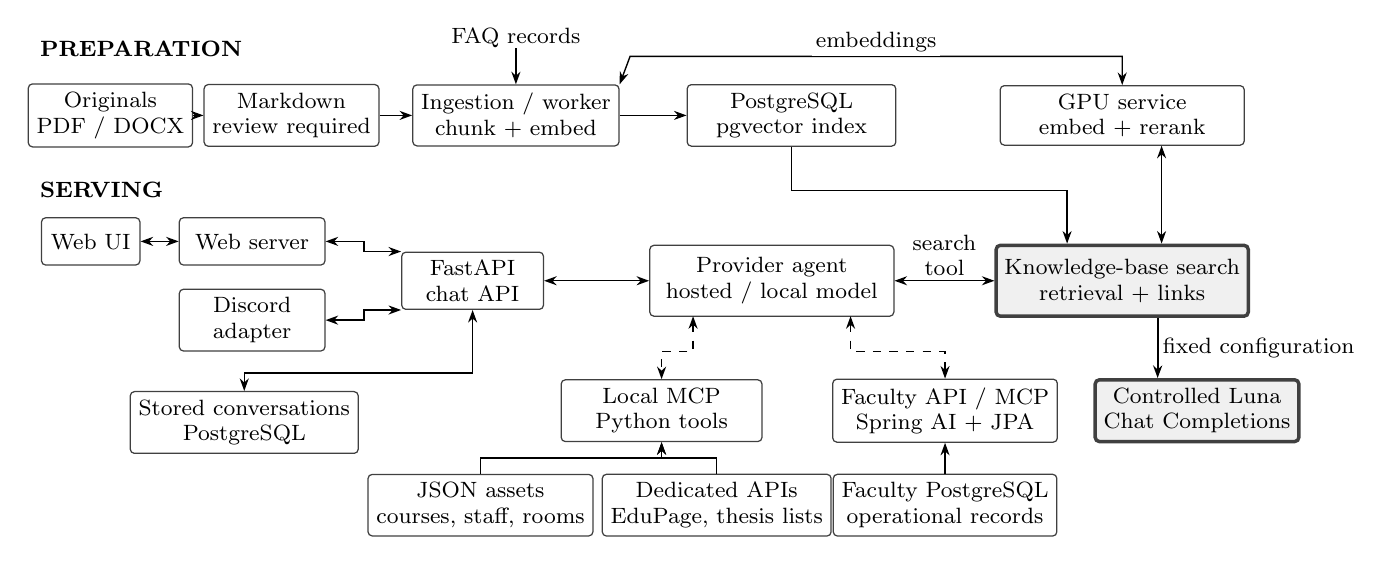
\begin{tikzpicture}[
  x=1cm,y=1cm,
  font=\fontsize{8}{9.2}\selectfont,
  box/.style={draw=black!75,line width=.45pt,rounded corners=1.5pt,
    fill=white,align=center,inner xsep=3pt,inner ysep=3pt,
    minimum height=.6cm},
  tested/.style={box,line width=1.25pt,fill=black!6},
  flow/.style={-{Stealth[length=1.6mm,width=1.15mm]},line width=.5pt},
  exchange/.style={arrows={{Stealth[length=1.6mm,width=1.15mm]}-{Stealth[length=1.6mm,width=1.15mm]}},line width=.5pt},
  optional/.style={exchange,dashed},
  note/.style={align=left,inner sep=0pt},
  edgeword/.style={fill=white,inner sep=1.5pt,align=center}
]
  % Preparation: archival originals are distinct from FAQ records.
  \node[note,font=\fontsize{8}{9.2}\selectfont\bfseries,anchor=west]
    at (0,.85) {PREPARATION};
  \node[box,minimum width=1.8cm] (originals) at (.9,0)
    {Originals\\PDF / DOCX};
  \node[box,minimum width=2.05cm] (markdown) at (3.2,0)
    {Markdown\\review required};
  \node[box,minimum width=2.55cm] (ingest) at (6.05,0)
    {Ingestion / worker\\chunk + embed};
  \node[box,minimum width=2.65cm] (vectors) at (9.55,0)
    {PostgreSQL\\pgvector index};
  \node[box,minimum width=3.1cm] (gpu) at (13.75,0)
    {GPU service\\embed + rerank};
  \draw[flow] (originals) -- (markdown);
  \draw[flow] (markdown) -- (ingest);
  \draw[flow] (ingest) -- (vectors);
  \node[note,anchor=south] (faq) at (6.05,.85) {FAQ records};
  \draw[flow] (faq.south) -- (ingest.north);
  \draw[exchange] (ingest.north east) -- (7.5,.75)
    -- node[edgeword,above] {embeddings} (13.75,.75) -- (gpu.north);

  % Serving: reply arrows denote request/stream exchanges, not shared state.
  \node[note,font=\fontsize{8}{9.2}\selectfont\bfseries,anchor=west]
    at (0,-.95) {SERVING};
  \node[box,minimum width=1.25cm] (web) at (.65,-1.6) {Web UI};
  \node[box,minimum width=1.85cm] (bff) at (2.7,-1.6)
    {Web server};
  \node[box,minimum width=1.85cm] (discord) at (2.7,-2.6)
    {Discord\\adapter};
  \node[box,minimum width=1.8cm] (api) at (5.5,-2.1)
    {FastAPI\\chat API};
  \node[box,minimum width=3.1cm,minimum height=.9cm] (agent)
    at (9.3,-2.1) {Provider agent\\hosted / local model};
  \node[tested,minimum width=3.1cm,minimum height=.9cm] (retrieval)
    at (13.75,-2.1) {Knowledge-base search\\retrieval + links};
  \draw[exchange] (web) -- (bff);
  \draw[exchange] (bff.east) -- (4.12,-1.6) |- (api.north west);
  \draw[exchange] (discord.east) -- (4.12,-2.6) |- (api.south west);
  \draw[exchange] (api) -- (agent);
  \draw[exchange] (agent) -- node[edgeword,above] {search\\tool} (retrieval);
  \draw[flow] (vectors.south) -- (9.55,-.95)
    -| ([xshift=-.7cm]retrieval.north);
  \draw[exchange] ([xshift=.5cm]gpu.south) -- ([xshift=.5cm]retrieval.north);

  % Stored conversations (web and Discord) are kept by the API.
  \node[box,minimum width=2.6cm] (store) at (2.6,-3.9)
    {Stored conversations\\PostgreSQL};
  \draw[exchange] (api.south) -- ++(0,-.8) -| (store.north);

  % Fixed configuration: retrieval, then prompt; the agent and tools are bypassed.
  \node[tested,minimum width=2.5cm] (luna) at (14.7,-3.75)
    {Controlled Luna\\Chat Completions};
  \draw[flow,line width=.8pt] ([xshift=.45cm]retrieval.south)
    -- node[edgeword,right] {fixed configuration} ([xshift=-.5cm]luna.north);

  % Structured records stay outside the FAQ/document embedding path.
  \node[box,minimum width=2.55cm] (localmcp) at (7.9,-3.75)
    {Local MCP\\Python tools};
  \node[box,minimum width=2.8cm] (facultymcp) at (11.5,-3.75)
    {Faculty API / MCP\\Spring AI + JPA};
  \draw[optional] (8.3,-2.55) -- (8.3,-3.0) -- (7.9,-3.0)
    -- (localmcp.north);
  \draw[optional] (10.3,-2.55) -- (10.3,-3.0) -- (11.5,-3.0)
    -- (facultymcp.north);
  \node[box,minimum width=2.6cm] (assets) at (5.6,-4.95)
    {JSON assets\\courses, staff, rooms};
  \node[box,minimum width=2.9cm] (adapters) at (8.6,-4.95)
    {Dedicated APIs\\EduPage, thesis lists};
  \node[box,minimum width=2.8cm] (facultydb) at (11.5,-4.95)
    {Faculty PostgreSQL\\operational records};
  \draw[flow] (assets.north) -- (5.6,-4.35) -| (localmcp.south);
  \draw[flow] (adapters.north) -- (8.6,-4.35) -| (localmcp.south);
  \draw[flow] (facultydb) -- (facultymcp);
\end{tikzpicture}}
\caption{Chatbot architecture and the components tested. In the deployed system the provider agent calls knowledge-base search and MCP tools itself (two-way arrows). Dashed arrows are MCP tools, which the controlled experiment did not evaluate. Bold border: the tested fixed retrieve-then-generate configuration, in which retrieval and prompt construction ran first and Luna answered, bypassing the agent and MCP tools. Structured-data lookup is separate from document and FAQ retrieval. GPU service: runs the embedding and reranking models. Web server: the backend of the web interface. Stream resumption and monitoring are omitted.}
\label{fig:architecture}
\end{figure*}


The \texttt{chat-bot} repository contains the Next.js web application, FastAPI backend and GPU service. The web server identifies the user, loads the conversation, sends limited history and model options to FastAPI, and displays the response stream. FastAPI checks access and request limits, assembles evidence, and calls a provider adapter. Application logic and storage run separately from GPU embedding and reranking.

The \texttt{discord-bot} repository connects Discord to the same API. Requests carry recent messages and \texttt{interface=discord} for formatting. The adapter streams answers, splits long messages and links feedback to response IDs. Its limited history stays in memory, while web conversations are saved in the database. It ignores separate source-information events, although URLs in answers remain visible. Web and Discord therefore use the same generation service but handle history and sources differently.

\subsection{Preparing and updating documents}
The \texttt{documents} repository stores original university PDFs/DOCX and their Markdown conversions. It extracts text where available and can transcribe scans with a vision model. The workflow requires checking conversions against the originals, but we could not confirm that every document had been reviewed. Uploading is a separate step: a client sends Markdown, a stable name, title and source information to the chatbot's document API. Optional R2 storage keeps the originals separate from the PostgreSQL retrieval index and the static feeds used by MCP.

The API hashes submitted content and splits Markdown into overlapping chunks at legal-article or section headings, keeping labels and order. Changed content replaces the document's chunks; separate endpoints accept short FAQ question/answer records. Indexing generates BGE-M3 vectors for PostgreSQL/pgvector. A worker can regenerate missing or outdated vectors after checking document revisions. Its status was not verified for every deployment.

Citation links use a supplied authority or source URL, falling back to the original file in the documents repository. An R2 storage key alone does not provide a citation link. Working copies add fields for source authority and whether a document is current. We have not confirmed that these fields are correctly filled in for the evaluated documents. The document version, extracted text and applicable rules need separate checks.

Email correspondence and PostHog questions are evaluation inputs and are not automatically added to the knowledge base. Request logs and saved conversations serve different purposes; general Discord commands, portal visits and scraper notifications must be distinguished from chatbot use.

\subsection{Selecting evidence and looking up records}
Retrieval merges dense candidates with lexical FAQ matches and ranks them with a GPU cross-encoder. It uses original or rewritten queries, applies score thresholds, prioritizes FAQs and adds neighboring chunks. The context and source-display thresholds are 0.10 and 0.30: a passage can reach the model without a visible source card. Provider adapters receive context, useful links, history and interface instructions, returning text, sources, response IDs and status events in a common format.

The Model Context Protocol (MCP) adds structured lookup. The generation agent can call tools discovered from configured servers after retrieval. The local Python server in \texttt{mcp} provides read-only searches for courses, staff, rooms, schedules and theses. It reads public JSON feeds; timetables and thesis catalogs use dedicated API or faculty-page adapters. The catalog UIs and MCP share these feeds and adapters, but we did not establish that scraped data automatically enters the retrieval index. Lexical FAQ expansion is a retrieval rule, separate from tool selection.

A separate Spring-based faculty API/MCP implementation exposes database records. Service authentication does not represent an individual student's permission to access private records. Read-only tools return records or links without submitting student transactions, allowing structured lookup without embedding every record. The inspected components differ in their tools and refresh behavior; the experiment does not test their availability or correctness.

\subsection{Request flow, reuse and evaluation scope}
For a procedural question, FastAPI retrieves FAQs and document passages, selects evidence and useful links, and builds the interface prompt. The provider agent generates an answer and may call tools. The adapter delivers the response; its ID links feedback and monitoring. A timetable question can use structured lookup, while an individual application may need clarification or referral. These are possible paths, not additional evaluated cases.

Another institution could reuse the source, retrieval and response interfaces while replacing local content, rules, tools, models and evaluation questions. This reuse has not been tested in a second implementation.

The retrieval-policy experiment uses 74 FAQs and 1,403 chunks from nineteen documents; the expanded collection used in the prompt comparison is described in Section~\ref{sec:followup}. Matching local and deployed file hashes identify the tested retrieval and prompt code. We use original queries without rewriting and exclude conversation history, access and request limits, storage, browser/Discord display and tools. Saved prompts go to Luna under fixed settings instead of the live provider agent. The test therefore covers only part of Figure~\ref{fig:architecture}.

\section{Controlled evaluation}
\subsection{Question sources and fixed sample}
The main sample contains 192 questions: 96 randomly selected representatives from the previously evaluated 320 email groups and 96 from 148 unique chatbot-question groups after normalization. Here, chatbot questions are those recorded in deployment logs. A separate 20-case email development sample is used for the pilot. Sampling uses seed 24905307 and does not use new answer-quality labels. Identifiers and hashes were fixed before generating the evaluated answers. The email cases had already been examined in earlier work, so they are not a previously unseen test set. Equal sample sizes make the two sources easier to compare, but do not reflect their frequency in actual use.

Chatbot questions come from the subset of requests with recorded message text. Of 699 requests in the observation period, 172 contain text; two extracted latest turns have no word tokens. The remaining 170 turns form 148 unique groups after normalization. All requests with recorded text are from July, while logs for newer retrieval policies appear later. We retain only the latest turn, so short follow-ups may be unclear without the preceding conversation. We group exact matches after standardizing the text; similar questions can still remain in separate groups.

Chatbot messages have a median length of 31.5 characters, compared with 306 in the earlier selected emails. Scripts also differ, but do not by themselves identify language. We report samples separately; their equal sizes do not represent actual use. Private questions remain local, and reported examples have personal details removed.

The application rejects four email questions above its 2,000-character limit. We keep their traces and all four policy records as input rejections, without shortening the questions or generating answers. Each sample and policy still counts all 96 questions, although only 92 email and 96 chatbot questions can proceed to generation. The 768 question--policy records therefore include sixteen input rejections and 752 eligible records before any later failures. Pilot cases are excluded from the main estimates.

\subsection{Policy comparison and fixed inputs}
Table~\ref{tab:factorial} lists the policies fixed before the experiment. G means a shared score threshold, S separate thresholds, and 0/1 fallback disabled/enabled. The main comparison is S0 minus G0; S1 minus G1 measures the threshold change with fallback enabled. G1 minus G0 and S1 minus S0 measure fallback effects. The thresholds were chosen during earlier development, without fitting them to the new answer outcomes.

\begin{table}[t]
\centering\small
\caption{Frozen two-factor comparison. Citation visibility remains 0.30 and the final candidate budget remains ten.}\label{tab:factorial}
\begin{tabular}{lrrc}
\toprule
Policy & FAQ min. & Doc. min. & Fallback\\
\midrule
G0 & 0.10 & 0.10 & Off\\
G1 & 0.10 & 0.10 & On\\
S0 & 0.10 & 0.00 & Off\\
S1 & 0.10 & 0.00 & On\\
\bottomrule
\end{tabular}
\end{table}

Fallback keeps the highest-scoring candidate only when no FAQ or document candidate passes its threshold. A separate recovery rule applies if the reranker fails: the application uses the vector-search order. We count that as an execution failure in this study. If a candidate already passes the lower document threshold, enabling fallback changes nothing. We check which policies produce identical contexts and how often fallback changes the input.

The evaluation program runs the actual retrieval function up to reranking, then saves the dense and lexical results, candidate order, source data and neighboring chunks. Each database transaction uses a consistent snapshot and cannot write data (read-only repeatable read). Separate batches may see different snapshots. The 9,329 saved candidate entries contain 681 unique IDs. Whenever an ID repeats, its text for reranking is identical. This check does not establish a single historical snapshot of the whole database. We import the deployed GPU modules in isolation to compute BGE-M3 query embeddings and BGE-reranker-v2-m3 scores~\cite{chen2024m3,baaiBgeRerankerV2M3}. Every policy reuses these results. Replay changes only the context-threshold comparison and the fallback condition in the production function.

Vector search with the original query keeps 31 candidates from each collection before merging them. Normally, lexical search can add FAQs only if the nearest scored FAQ is at least as close as the nearest scored document, or there is no scored document. If a transliterated query is also available, a scored candidate from either collection is enough. Candidates equal to the threshold are kept. FAQs receive priority within the final ten-candidate limit. Each selected document chunk gains one neighbor on each side. Overlapping groups merge in document order and keep the earliest selected rank. Source visibility stays at 0.30. Useful-link reranking is saved separately and held fixed. Only the two policy settings vary.

\subsection{Generation and execution controls}
The application's \texttt{handle\_chat} function builds the system and user prompts with \texttt{interface=web}, wording for empty retrieval, useful links and a fixed date of 07.09.2026. We intercept generation and send the exact captured prompts to Luna through Chat Completions. Production uses a Responses/agent path, so the experiment does not test live tools or establish that defaults are equivalent across the two paths.

For the requested \texttt{gpt-5.6-luna} alias, the gateway reports \texttt{gpt-5.6-luna-2026-07-09}. We record this identity without independently verifying the underlying model. Generation uses reasoning effort none, a 1,024-token limit, no automatic retry and the gateway's default sampling settings. The application's temperature and top-$p$ are saved as metadata but are not sent in these requests.

When questions, prompts and settings are identical, including the exact prompt bytes, policies reuse one generated answer. Unique requests are shuffled with a fixed seed. Reusing an answer does not provide another independent observation. Failures, truncation and invalid assessments remain in the results. Usage and timing describe actual provider calls, excluding the rest of the browser interaction.

Capture and replay block application HTTP requests and database writes. The plan, deployment versions, frozen references, full source hashes and exact prompts are saved in \path{research/luna_evaluation}; the prompt comparison uses \path{research/effectiveness_v2}.

\section{Assessment and analysis}
\subsection{Reference construction and answer assessment}
Before generating the evaluated answers, Luna builds a reference describing what an answer to each question should cover. All policies use the same reference, which is prepared without seeing their answers. The source pool alternates between up to eight FAQs and eight document chunks, each group ordered by score. Each source contributes at most its first 1,400 characters, within a 12,000-character total. This limited pool favors material found by retrieval and may miss evidence needed to answer the question. The references have not been approved as correct answers by the institution.

References record answerability, required facts and quotations, actions, currentness and uncertainty. Code checks quotation occurrence in the named source. Failed facts remain in raw outputs but leave the checked fact list, and the reference becomes uncertain. An otherwise positive answer or routing judgment then becomes uncertain; negative and incomplete outcomes remain. Of 212 pilot and main references, 182 pass. This rule prevents failed references from establishing success, but does not prove meaning or currentness. Empty fact lists can also pass.

The primary judge sees one anonymous answer, its question, the shared reference and the exact generation prompt. It does not see policy labels or earlier judgments. It returns an overall category, an explanation and evidence quotations. Separate fields, called \emph{flags}, report whether material claims lack support, required facts are covered and citations support the answer. A record is \emph{structurally valid} if its format is correct and its fields pass consistency checks. For example, it cannot report success while flagging an unsupported material claim. Passing these checks does not mean that the judge found every claim or interpreted every quotation correctly.

A \emph{material claim} concerns matters such as eligibility, fees, deadlines, procedure or completion of an administrative task. An unsupported-material-claim flag requires the unsupported category; inconsistent judgments fail structural validation. A supported answer must include the required facts and their conditions. \emph{Useful safe routing} means asking for necessary clarification, directing the user to verify information or referring them to staff, without claiming to have completed a private transaction. Missing content, unnecessary refusal to answer, uncertain evidence, and execution or assessment failures are separate outcomes. An incorrect displayed citation prevents strict success even if the answer otherwise seems plausible.

\subsection{Calibration, pilot, and sensitivity}
We check the assessment procedure with 18 AI-authored examples based on source documents. They cover contradictions, omissions, incorrect citations, fabricated transactions, justified refusal and limits on applicability. A documented addendum adds twelve Macedonian examples arranged as six Cyrillic/Latin pairs. These development checks have not been independently validated and do not represent a user study. All eighteen original records are structurally valid; seventeen match the expected category and all eighteen match the material-claim flag. In the remaining case, the judge labels useful routing as a supported answer. All twelve script examples match both expected categories and material flags, although each pair represents the same task. We kept the settings and assessment rules unchanged. These checks cannot remove judge bias from the estimates.

The 20-case pilot completed 39 unique generations, with 38 structurally valid assessments and one retained failure. We then proceeded with the fixed settings and assessment rules. The pilot confirmed that the pipeline ran; it did not establish assessor accuracy.

Luna builds the references, generates the answers and supplies the primary judgments. Errors may carry across these stages, and the judge may favor its own model's answers. We repeat 48 unique answer assessments, selected with a fixed seed: 41 main-study and seven pilot answers. We also assess this subset with a fixed local version of Qwen3-8B Q4\_K\_M~\cite{yang2025qwen3}, temperature zero, a 1,024-token limit, a 90-second timeout and no retry. We report invalid outputs, exact agreement and kappa where defined. An additional check uses saved outputs to compare whether the judges label each answer as assistance after reference validation. It keeps main and pilot answers separate. Shared references reveal disagreement, not correctness.

\subsection{Outcome measures and denominators}
For question $i$ and policy $p$, let $Y_{ip}$ indicate an AI-assessed supported answer or useful safe routing. We also report these two outcomes separately, alongside unsupported material claims. Within each question sample, the primary paired difference is
\[
\widehat{\Delta}_{\mathrm{threshold}}=
\frac{1}{96}\sum_{i=1}^{96}(Y_{i,\mathrm{S0}}-Y_{i,\mathrm{G0}}).
\]
Input rejection, generation failure, unusable assessment and uncertainty count as unsuccessful outcomes. Any additional estimate based only on completed answers with usable assessments must state how many answers it includes.

The interaction measures whether fallback has a different effect under the two threshold settings. In percentage points, it is $(\mathrm{S1}-\mathrm{S0})-(\mathrm{G1}-\mathrm{G0})$. We estimate confidence intervals by resampling question groups 20,000 times with seed 24905310, keeping each question's policy results together. These bootstrap intervals show how the estimates vary across question samples while the AI labels stay fixed. They do not account for systematic judge error. Reused answers stay linked to every policy record they represent. Combined summaries describe only the balanced sample; email and chatbot results keep separate denominators.

To explain policy effects, we measure empty contexts, cases where fallback changes the context, the mix and overlap of selected sources, and context length. More text does not by itself mean more relevant evidence. We report provider response times and usage-based cost estimates separately from answer outcomes. Planning rates are not verified gateway charges or total system costs.

\section{Results}
\subsection{Assistance outcomes and retrieval comparison}
Table~\ref{tab:luna-outcomes} separates answering from guidance. Under G0, assistance labels cover 31/96 email responses: nine supported answers and 22 useful-routing responses. The 53/96 chatbot responses include 25 supported answers and 28 useful-routing responses. Many positive labels therefore describe a useful next step rather than a complete factual answer. These are AI judgments on the selected questions, not verified success rates for all users.

The reference check has an important limitation: 76 of the 182 passing references contain no retained facts. In the main sample, 75 of 166 passing references are empty: twelve email and 63 chatbot cases. Twenty of the 25 chatbot supported-answer labels under both G0 and S0 use such references. The judge can mark all required facts as covered even when there is no fact to check. Greetings, explanations of the assistant's abilities and clarifications may still be useful, but these labels do not establish factual accuracy.

A post-hoc sensitivity analysis applies a stricter rule: count a supported answer only if its reference passes validation and contains at least one fact. Safe routing still counts as assistance. Email totals become 31/96 under G0 and 29/96 under S0, a $-2.1$-point difference (95\% interval $[-9.4,5.2]$). Chatbot totals become 33/96 and 32/96, a $-1.0$-point difference ($[-7.3,5.2]$). The original primary measure stays unchanged. This is not an accuracy correction: the stricter rule also excludes potentially useful replies that need no factual answer.

All 192 main questions have four replay records. Of 768 outcomes, 752 are eligible for generation and use 354 unique answers; the remaining eligible records reuse those answers. All 354 main generations completed within the output limit. Sixteen policy outcomes are input rejections. Another twelve have invalid assessments, representing six unique judgments. All six flag an unsupported material claim. Since these assessments are invalid, we keep them as failures without accepting or repairing their verdicts. No main references, replay records or primary outcomes are missing. Tables~\ref{tab:luna-outcomes} and~\ref{tab:luna-effects} keep the full sample denominators.

% Data from research/luna_evaluation/generated_tables.tex; presentation edited for clarity.
% Intervals are percentage points conditional on AI labels.
\begin{table*}[t]
\centering\small
\setlength{\tabcolsep}{5pt}
\caption{AI-assessed outcomes (fixed pipeline, not the deployed settings). Each sample and policy keeps all 96 selected cases. Answer is the judge's supported-answer label and can include conversational replies. It is not verified factual accuracy, because 20 of the 25 chatbot Answer labels under the baseline and the lower floor use references with no facts after the check.}
\label{tab:luna-outcomes}
\begin{tabular}{llrrrrrrrr}
\toprule
Sample & Policy & $N$ & Answer & Route & Unsup. & Incomp. & Refusal & Uncert. & Fail \\
\midrule
Email & Baseline & 96 & 9 & 22 & 20 & 31 & 0 & 9 & 5 \\
Email & Baseline + fallback & 96 & 9 & 23 & 25 & 23 & 0 & 12 & 4 \\
Email & Lower floor & 96 & 10 & 20 & 19 & 30 & 0 & 10 & 7 \\
Email & Lower floor + fallback & 96 & 10 & 20 & 19 & 30 & 0 & 10 & 7 \\
Chatbot logs & Baseline & 96 & 25 & 28 & 12 & 22 & 4 & 4 & 1 \\
Chatbot logs & Baseline + fallback & 96 & 25 & 27 & 11 & 24 & 4 & 3 & 2 \\
Chatbot logs & Lower floor & 96 & 25 & 27 & 11 & 24 & 4 & 4 & 1 \\
Chatbot logs & Lower floor + fallback & 96 & 25 & 28 & 11 & 23 & 4 & 4 & 1 \\
\bottomrule
\end{tabular}
\par\smallskip\begin{minipage}{0.94\textwidth}\footnotesize Assistance combines Answer and Route (useful clarification or referral). Unsup.: unsupported material claim. Incomp.: incomplete. Refusal: unnecessary refusal. Uncert.: uncertain. Positive judgments count as uncertain when reference validation fails. Fail includes input rejection, generation failure and invalid assessment. All expected outcome records are present.\end{minipage}
\end{table*}
\begin{table}[t]
\centering\footnotesize
\setlength{\tabcolsep}{3pt}
\caption{Paired assistance differences in percentage points for the fixed pipeline (not the deployed settings), with 95\% bootstrap intervals from 20,000 resamples of question groups. The AI labels stay fixed, so the intervals do not correct judge error.}
\label{tab:luna-effects}
\begin{tabular}{lrr}
\toprule
Comparison & Email & Chatbot logs \\
\midrule
Lower floor vs.\ baseline & -1.0 [-8.3, 6.3] & -1.0 [-7.3, 5.2] \\
Same, with fallback & -2.1 [-9.4, 5.2] & 1.0 [-4.2, 6.3] \\
Fallback, baseline & 1.0 [-4.2, 6.3] & -1.0 [-7.3, 5.2] \\
Fallback, lower floor & 0.0 [0.0, 0.0] & 1.0 [0.0, 3.1] \\
Interaction & -1.0 [-6.3, 4.2] & 2.1 [-3.1, 8.3] \\
\bottomrule
\end{tabular}
\par\smallskip\begin{minipage}{0.98\columnwidth}\footnotesize For email, adding the fallback to the lower floor uses identical contexts and reused answers for every question, so its zero-width interval says nothing general about equivalence. Estimates and intervals use one decimal place (6.25 is printed as 6.3).\end{minipage}
\end{table}


Under S0, assistance totals change to 30/96 for email and 52/96 for chatbot logs. The paired difference is $-1.0$ percentage points in each sample. The 95\% interval is $[-8.3,6.2]$ for email and $[-7.3,5.2]$ for chatbot logs. Both allow meaningful improvement or decline. We cannot conclude that the lower threshold improves assistance or that the policies are equivalent.

With fallback enabled, lowering the document threshold changes assistance by $-2.1$ points for email and $+1.0$ for chatbot logs. Under the shared threshold, adding fallback (G1 versus G0) changes empty contexts to nonempty ones in 33 email and 27 chatbot cases, with outcome differences of $+1.0$ and $-1.0$ points. Under the lower document threshold, S0 and S1 select identical contexts and source IDs for all 96 email questions; only three chatbot contexts change, with a one-case outcome difference. Fallback therefore changes few contexts in S0 versus S1, but many under the shared threshold. We counted these changes by comparing contexts; we did not record directly which code branch ran. Interaction estimates are $-1.0$ and $+2.1$ points, with intervals spanning zero.

Under G0 and S0, the judge identifies unsupported material claims in twenty and nineteen email outcomes, and twelve and eleven chatbot outcomes. Under G1, the count rises to 25 for email and falls to eleven for chatbot logs. These counts use the full samples, with uncertainty and failure reported separately. The apparent email decline from twenty to nineteen is not clear evidence of safer answers: judgments with a specified material-claim flag fall from 91 to 88, while invalid judgments with a raw unsupported-claim flag rise from one to three. Those invalid flags are retained for inspection, not accepted as verdicts. Incomplete answers remain common under G0 and S0: 31/96 and 30/96 for email, and 22/96 and 24/96 for chatbot logs.

The retrieved context changes much more than the assistance scores. For email, moving from G0 to S0 reduces empty contexts from 36 to three, increases mean context length from 5,110 to 16,481 characters, and raises the mean number of selected document candidates from 0.82 to 6.67. For chatbot logs, empty contexts fall from 76 to 52 and mean length rises from 1,010 to 5,808 characters. These counts exclude the useful-link catalog added separately to the prompt, so an empty retrieval block can still be accompanied by useful links. Differences between the samples cannot be attributed solely to language or script.

One G0 answer misses steps needed after an exam-registration deadline. The student asked for help registering late. The answer declined to perform registration, described ordinary iKnow registration and mentioned a penalty. The saved FAQ describes a separate request for each exam, naming the course and session. It then asks the student to notify Student Services after payment. These steps were missing from both the answer and its G0 context, but were present in the broader reference pool. The answer leaves the next step unexplained; the source does not establish whether late registration is currently allowed. The selection list contained 36 incomplete G0 cases whose references passed validation and contained facts. An AI reviewer followed the fixed order and rejected ten cases before selecting this one. The example has personal details removed. It shows an omission against a saved source, not how often this happens or human-validated correctness.

We also check whether validated reference quotations appear in the retrieval context. Among 66 email cases with valid nonempty reference facts, the mean proportion of quotations found per case rises from 0.486 under G0 to 0.661 under S0. All quotations are present in eighteen versus 29 cases. This checks exact text matches. It does not tell us whether all relevant information in the collection was found. Taken with the answer outcomes, it shows that adding potentially useful passages does not necessarily produce more complete or better-supported answers.

In the main sample, 78/96 email and 88/96 chatbot references pass the quotation check. The reference-validation rule changes 47 success labels to uncertain across policies: 32 email and fifteen chatbot records, representing 28 unique judgments. Under G0 versus S0, these counts are seven versus eight for email and four versus four for chatbot logs. The 47 records can count the same failed reference check under several policies because those policies reuse a judgment. The saved raw judgments allow the effect of this rule to be checked.

An offline diagnostic searches the saved evidence pools for the 49 rejected main-reference quotations. Of these, 32 occur in a different source block and seventeen are absent from the pool. The matches suggest possible source-ID corrections, but still require checks of meaning and applicability. No references or outcome labels were changed.

Median provider-call latency is 2.144 seconds for email and 1.466 seconds for chatbot logs; the 95th percentiles (p95) are 3.439 and 3.854 seconds. Main generation costs an estimated USD~5.43 at planning rates of USD~2 per million input and USD~12 per million output tokens. This excludes preparation, assessment, diagnostics, GPU computation and hosting, and is not a verified invoice.

\subsection{Assessment sensitivity}
Across the 48-answer subset, repeated Luna produces 47 valid judgments. The primary and repeat fail on the same answer. Categories agree in 35/47 pairs (74.5\%, $\kappa=0.648$); specified material-claim flags agree in 40/46 (87.0\%, $\kappa=0.340$). Most flags are negative, increasing chance agreement and lowering kappa relative to percentage agreement.

Qwen produces 46 valid records and two consistency failures. With the invalid primary judgment excluded, categories agree in 13/45 pairs (28.9\%, $\kappa=0.134$), material flags in 20/44 (45.5\%, $\kappa=0.104$), and citation flags in 14/32. Qwen flags unsupported claims in 23 pairs where Luna does not; the reverse occurs once. Hashes confirm identical questions, references, answers and prompts, but models, sampling and numerical precision differ. Qwen's labels are not known to be correct; disagreement limits confidence in the scores.

An assistance check excludes pilot answers and applies the original reference rule to both judges. Repeated Luna agrees in 38/40 usable pairs from 38 cases (95.0\%): one gain and one loss leave fourteen assistance labels in each run. Qwen agrees in 25/38 pairs from 37 cases (65.8\%): nine losses and four gains reduce assistance from thirteen to eight. The shared rule can raise agreement by removing positives from both judges, while still accepting empty references. Some questions contribute multiple answers, and not all policies are covered. This check neither identifies the correct judge nor recalculates the full policy effect.

On the thirty unchanged controls, Qwen returns valid outputs but matches expected categories and material flags on only 14/18 original and 10/12 script examples. All six mismatches treat missing information, routing or unnecessary refusal as unsupported claims. This helps explain its harsher labels without proving Luna correct. The controls are AI-authored, script versions are paired, and no primary labels or rules change.

\subsection{Expanded collection and prompt comparison}\label{sec:followup}
The prompt comparison uses a separate read-only snapshot with 74 FAQs, sixty documents and 2,391 chunks. FAQ text is unchanged. Captured candidate and neighboring-chunk text matches the snapshot, and the documents repository is separately pinned. The retrieval-policy experiment is unchanged; differences between the two experiments cannot be attributed to corpus growth alone.

A 32-question development sample, balanced between email and chatbot sources and selected across earlier reference states, compares current retrieval, AI-selected reference evidence and no evidence. Selected evidence raises fact coverage from 29/73 to 50/73 and strict completion from 4/32 to 6/32. No reference establishes full factual answerability, so this difficult-case diagnostic is neither representative nor a perfect-evidence upper bound. The judge also lacked parts of the generation evidence, limiting absolute diagnostic scores.

Budget was allocated to the first forty emails in a shuffled 64-question reserve before reference preparation; 24 cases retain retrieval captures only. Previously evaluated exact and near-duplicates were excluded, but the reserve was screened earlier and semantic independence is unproved. Two AI passes prepare and review references before generation. Selecting source lines avoids quotation-transcription errors. All forty references pass exact-text checks: 34 partial, three insufficient and three nonfactual. They are not institution-approved answers.

We freeze a prompt-only change after development: check dates and applicability instead of automatically favoring FAQs or earlier-ranked text, preserve needed procedural steps, and clarify material gaps. Conditions share production retrieval with fallback enabled, useful links, Luna, gateway sampling defaults and a 1,536-token cap. Three oversized inputs remain in each forty-question denominator. Strict completion requires all reference facts and behaviors, no unsupported claim or citation error, and no reference concern. Empty factual/mixed references cannot establish success. These requirements differ from the original assistance measure.

The initial judge lacked some generation evidence and flagged fifteen citation errors per condition, although a deterministic check found only one answer per condition with a URL absent from the generator's context and links. URL absence does not establish a broken link. A post-hoc audit of all pairs supplied the full generation context, revised scope guidance and reduced the judgment cap to 1,024 tokens. Changes cannot be attributed to added context alone; original judgments remain unchanged.

\begin{table}[t]
\centering\small
\caption{Forty-question prompt comparison. Audit: post-hoc assessment with the actual generation evidence.}\label{tab:followup}
\begin{tabular}{lrr}
\toprule
Measure & Current & Revised\\
\midrule
Completed generations & 37/40 & 37/40\\
Initial strict completions & 4/40 & 6/40\\
Audit strict completions & 6/40 & 5/40\\
Audit unsupported-claim flags & 15/37 & 10/36\\
Audit citation-error flags & 1/37 & 1/36\\
\bottomrule
\end{tabular}
\end{table}

The audit difference is $-2.5$ points (95\% paired bootstrap interval $[-12.5,7.5]$; 20,000 resamples): two gains and three losses. One revised-condition judgment has an invalid source span and remains a failure. Flag denominators count valid judgments only (Table~\ref{tab:followup}). Partial references, unnecessary requirements and source uncertainty limit interpretation. Completion can mean guidance with stated gaps; fewer unsupported-claim flags do not establish overall improvement.

Before the audit, repeated Luna judgments agreed on strict completion in 37/40 answer pairs from twenty randomly selected questions. Both runs shared the incomplete evidence. Eight constructed controls matched expected outcomes, but do not validate real-case references. Separately, deployed prompt assembly preserved the available history in six saved user turns, and read-only MCP functions returned staff/course lists and an exact staff lookup. These are component checks, not tests of full conversations or agent tool selection.

\subsection{Deployment observations}
Saved deployment logs cover 28 June 2026 through 5 September 2026, including the first date and excluding the last. Events explicitly marked as basic system tests were removed. The logs record 699 API requests and 684 generation events: 651 labeled completed, seventeen empty and sixteen disconnected. Completed events have a median duration of 12.154 seconds and p95 of 37.225 seconds. Timing starts after the application resolves credentials, so it does not capture the user's full wait. Request and generation records cannot always be linked. An error after partial output can also keep a completed label. These counts therefore cannot provide a verified success rate.

The logs sometimes use response IDs in place of user IDs, so they cannot reliably count unique students. Recorded use is concentrated, and 37 feedback events refer to only sixteen responses. Repeated feedback may reflect changes of opinion, so these events cannot establish satisfaction. Selective message logging supplied real questions for the chatbot sample, but does not make that sample representative. The logs show recorded activity; they do not label answer-quality outcomes for the new experiment.

\section{Discussion and limitations}
\textbf{RQ1: useful guidance differs from a complete answer.} Routing accounts for more positive outcomes than supported answering under G0 in both samples. Explaining where to seek help may be useful while leaving the question unanswered. Incomplete answers and unsupported claims remain common. The failure example shows why ordinary instructions may not help when a student misses a deadline. Empty references and unverified judgments prevent treating the totals as established accuracy.

\textbf{RQ2: more context did not clearly improve assistance.} Lowering the document threshold adds passages and reference quotations without clearly improving outcomes. Fallback shows no clear benefit, and the revised prompt's apparent gain does not survive reassessment. Neither experiment identifies a generally better configuration; plausible fixes still require controlled outcome checks.

\textbf{RQ3: conclusions depend on the questions and judge.} Samples differ in length, history, selection and previous use. Repeated or different judges disagree without establishing correctness. Shared models, limited references and empty fact lists weaken estimates. Exact quotations and valid formatting do not prove that evidence supports an answer.

Source authority also needs attention. Transfer rules in the faculty (2013) and university (2019, supplemented 2022) rules cover different situations~\cite{finki2013study,ukim2019study,ukim2022supplement}; the institution must determine which rule applies. The fee schedule applies from 2024/25 until it is replaced~\cite{finki2024fees}. A document's upload date is not necessarily the date it took effect. Retrieving its text accurately cannot, by itself, determine an individual's eligibility, fees or completion of an administrative process.

The study tests answers to the latest message without earlier conversation history. A referral does not show that the problem was resolved, and delivery logs cannot validate answer quality. Administrative workload, avoided emails and staff-time savings are outside scope.

The judge must receive the evidence available to the generator. Reported substantive inaccuracies also require auditing official faculty and university information with responsible staff. Complete conversations should be reviewed to identify missing knowledge and distinguish it from retrieval failures, guiding source collection and correction. Full-conversation answers and tool selection still require outcome evaluation beyond component checks.

\textbf{Data use and reproducibility.} Correspondence and logs were used with permission. Private questions, answers and reviews remain local. Saved code, prompts and records allow recalculation, but gateway defaults and model availability limit exact regeneration. The retrieval-policy experiment lacks a complete historical database snapshot; the prompt comparison retains one. No public dataset release is claimed.

\section{Conclusion}
The chatbot aims to give supported answers and useful guidance when it cannot answer directly. The 192-question retrieval comparison finds frequent omissions and no clear benefit from more context. A separate forty-question prompt comparison also fails to establish improvement after an assessment audit. The architecture links these findings to source preparation, retrieval and delivery. The evaluations identify concrete gaps, including incomplete judge inputs, but do not establish verified factual accuracy or full-system effectiveness. Further work should verify official information, identify missing knowledge through conversation review, and establish reliable answer references.

\bibliographystyle{plain}
\bibliography{references}
\end{document}
